%% Original author:
%% © unknown
%%
%% Modified by:
%% © 2016 KH1
%%
%% This file belongs to the architecture project. See the LICENSE
%% file for more detail on copying.
%%

\documentclass[
12pt,
french,                           % 
a4paper,
]{article}




%
% TYPESETTING FRENCH -- FONTS
%
  \usepackage{lmodern, textcomp}
  % textcomp provides more mappings between utf8 chars and font chars


% Additional symbols
%\usepackage{amssymb,amsmath}
\usepackage{ifxetex,ifluatex}

% Choose font according to driver
\ifnum 0\ifxetex 1\fi\ifluatex 1\fi=0 % if pdftex
  \usepackage[T1]{fontenc}
  \usepackage[utf8]{inputenc}
  \DeclareUnicodeCharacter{20AC}{\texteuro}
  \else % if luatex or xelatex
  \ifxetex
    \usepackage{mathspec}
    \usepackage{xltxtra,xunicode}
  \else
    \usepackage{fontspec}
  \fi
  \defaultfontfeatures{Mapping=tex-text,Scale=MatchLowercase}
  \newcommand{\euro}{€}
        \fi

% Babel
\ifxetex
  \usepackage{polyglossia}
  \setmainlanguage{french}
\else
  \usepackage[french]{babel}
\fi

% use microtype if available
\IfFileExists{microtype.sty}{%
  \usepackage{microtype}
  \UseMicrotypeSet[protrusion]{basicmath} % disable protrusion for tt fonts
}{}





%
% LAYOUT
%

% Hyperref
\ifxetex
  \usepackage[setpagesize=false, % page size defined by xetex
              unicode=false, % unicode breaks when used with xetex
              xetex]{hyperref}
\else
  \usepackage[unicode=true]{hyperref}
\fi
\hypersetup{breaklinks=true,
            bookmarks=true,
                        colorlinks=true,
            pdfborder={0 0 0}}
\urlstyle{same}  % don't use monospace font for urls

% Headers
\usepackage{fancyhdr}
\pagestyle{fancy}
\pagenumbering{arabic}
\lhead{}
\chead{}
\rhead{\itshape{\nouppercase{\leftmark}}}
\lfoot{v 0.2.0}
\cfoot{}
\rfoot{\thepage}



%
% SPECIAL PAGES
%
% Tables

\usepackage{graphicx,grffile}
\makeatletter
\def\maxwidth{\ifdim\Gin@nat@width>\linewidth\linewidth\else\Gin@nat@width\fi}
\def\maxheight{\ifdim\Gin@nat@height>\textheight\textheight\else\Gin@nat@height\fi}
\makeatother
% Scale images if necessary, so that they will not overflow the page
% margins by default, and it is still possible to overwrite the defaults
% using explicit options in \includegraphics[width, height, ...]{}
\setkeys{Gin}{width=\maxwidth,height=\maxheight,keepaspectratio}



%
% PARAGRAPH FORMATTING
%
\setlength{\parindent}{0pt}
\setlength{\parskip}{6pt plus 2pt minus 1pt}
\setlength{\emergencystretch}{3em}  % prevent overfull lines
\usepackage{enumerate}
\providecommand{\tightlist}{%
  \setlength{\itemsep}{0pt}%
  \setlength{\parskip}{0pt}%
}
\setcounter{secnumdepth}{5}

% Redefines (sub)paragraphs to behave more like sections
\ifx\paragraph\undefined\else
\let\oldparagraph\paragraph
\renewcommand{\paragraph}[1]{\oldparagraph{#1}\mbox{}}
\fi
\ifx\subparagraph\undefined\else
\let\oldsubparagraph\subparagraph
\renewcommand{\subparagraph}[1]{\oldsubparagraph{#1}\mbox{}}
\fi


%
% DOCUMENT
%
\title{ Le réseau de distribution de gaz de GrDF - Projet de structuration }
\author{ Mohammed Amiri\and Philémon Pensier \and Romain Milville}
\date{14 janvier 2016}

% 0 - header before document

\begin{document}
% 1 - title page

\clearpage

% 2 - abstract

% 3 - forematter

% 4 - tables of content
{
  \hypersetup{linkcolor=black}
  \setcounter{tocdepth}{3}
  \tableofcontents
}


% 5 - mainmatter
\clearpage
\section{Intruduction}

Le présent rapport présente la structuration et la modélisation d'un
système de distribution de gaz du point de vue de GrDF. L'UML (Unified
Modeling Language) sera le principal outil utilisé.

Plusieurs points du système de distribution de gaz seront abordés :

\begin{itemize}
\item
  Le réseau en lui-même, comment-il organisé, géré, maintenu\ldots{} ?
\item
  La mise en sécurité, comment gérer les alertes pour problème sur le
  réseau ?
\item
  Enfin, le système de comptage avec notamment le nouveau système de
  compteur communiquant Gazpar.
\end{itemize}

\section{Présentation de GrDF}

GrDF est une entreprise de distribution de gaz. Sa mission est
d'acheminer le gaz afin que des personnes ou des entreprises puissent
s'en servir comme énergie. Pour autant, GrDF ne doit pas être confondu
avec un fournisseur de gaz qui est un entreprise qui vend le gaz à des
clients. Il y a ainsi entre GrDF et les fournisseurs la même relation
qu'il y avait entre la SNCF et RFF :

GrDF se sert du réseau pour acheminer le gaz qui appartient aux
fournisseurs vers leurs client. Les fournisseurs payent GrDF en échange
proportionnellement à l'énergie utilisé par les usagers.

Le prix payé par unité d'énergie consommé est fixé par la commission de
régulation de l'énergie (CRE). Ce système a été mis en place afin de
garantir une concurrence loyale entre les fournisseurs.

Pour autant, avant 2004, EDF-GDF assurait à la fois la distribution et
le service clientèle. En 2004, EDF et GDF deviennent deux identité
distinctes et à partir de 2007 GDF et GrDF sont séparés afin de donner
libre concurrence aux différents fournisseurs. Aujourd'hui GrDF est une
filiale d'ENGIE à 100 \% et compte environ 11 000 employés. Le siège
d'ENGIE se trouve à Courbevoie à La Défense.

Le réseau est composé d'un appareillage complexe, le schéma suivant
montre un exemple de porion de réseau où chaque type d'appareillage
apparaît. Il montre ainsi comment cet appareillage s'organise.

\begin{figure}[htbp]
\centering
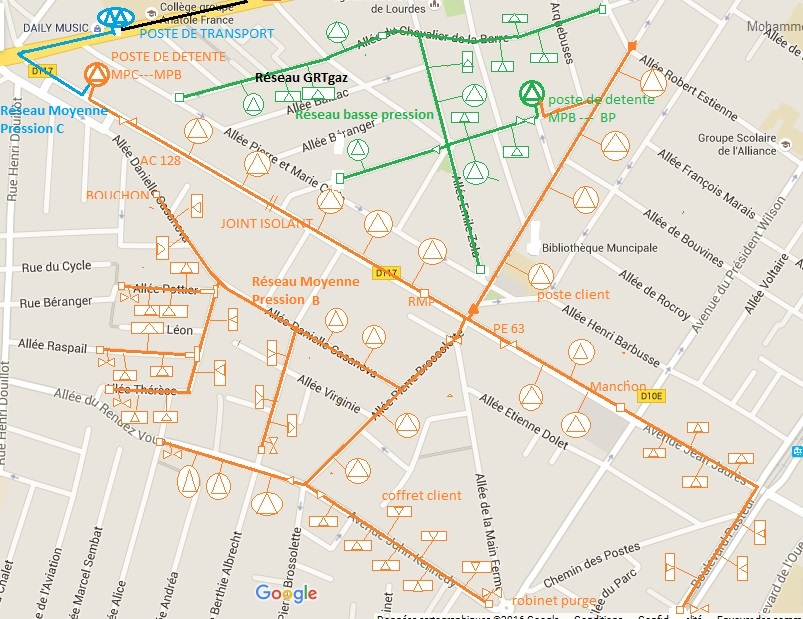
\includegraphics{carte_gaz.jpg}
\caption{alt text}
\end{figure}

Sur ce schéma, on observe d'abord plusieurs type de pression pour les
canalisation (couleurs différentes). Ceci n'a pas d'impact sur chaque
type d'appareillage.

Il existe plusieurs types de canalisations :

\begin{itemize}
\item
  Les canalisations en cuivre, Ce type de matériau a été très peu
  utilisé en raison de sa faible résistance au choc. Environ 20 km sont
  enregistrés dans le fichier patrimonial de GrDF. La pose a été
  réalisée majoritairement dans les années 1960. Les canalisations
  cuivre ont été utilisées pour réaliser des parties peu importantes des
  réseaux en moyenne pression B (MPB). L'arrêté du 13 juillet 2000 ne
  prévoit plus l'utilisation des canalisations cuivre.
\item
  Les canalisations en acier. Elles sont utilisées depuis 1931 et ont
  surtout été utilisées dans les années 70/80. Ces canalisations sont
  munies de systèmes de protection cathodique pour éviter leur
  corrosion. On a deux types de protection, d'une par la protection
  passive correspondant à l'enrobage de la canalisation dans une
  substance isolante, d'autre part on a des protections actives qui
  correspondent à la mise en place d'anodes sacrificielles qui vont
  drainer les courants vagabonds et corriger le potentiel
  électrolytique.
\item
  La canalisation en polyéthylène (PE). Elles se sont généralisées à
  partir des années 80. Ce sont en général des canalisations en moyenne
  pression B. Le succès de cette matière s'explique par la simplicité de
  mise en œuvre. En effet le PE permet l'utilisation de tubes de grandes
  longueurs et un raccordement des tubes par électrosoudage . Le PE est
  maintenant utilisés systématiquement pour l'installation de
  canalisations ayant une pression de moins de 10bars.
\item
  Les canalisations en fonte ductile. Elles sont utilisées depuis la
  mise en place du réseau de gaz. Elle sont utilisées pour le réseaux
  basse pression (BP). Ce sont les réseaux qui irriguent les centres
  villes, ils sont l'héritage des réseaux manufacturés. Un arrêté du 13
  juillet 2000 portant sur la sécurité des réseaux de gaz ne prévoit
  plus la mise en place de telles canalisations et les réseaux BP sont
  progressivement remplacés par des réseaux moyenne pression B (de 4
  bars)
\end{itemize}

Parmi l'appareillage du réseau on a :

\begin{itemize}
\item
  Les postes de détente. Ils permettent le changement de pression. Il y
  en a de plusieurs type, d'abord on a les postes de livraison qui font
  le lien entre le réseau de transport de GRT Gaz et GrDF. On a ensuite
  les poste de détente de concession qui permettent le changement de
  pression pour permettre l'utilisation du gaz.
\item
  Les robinets et vannes. Ils permettent d'arrêter la fourniture en cas
  d'incident.
\item
  Les manchons. Ils permettent le raccordement de plusieurs tubes de
  canalisation.
\item
  Les compteurs. Ces derniers permettent de connaître le volume de gaz
  consommé par un poste client dans le but de pouvoir facturer au plus
  juste.
\item
  Des cônes réducteur. Ils permettent la diminution du diamètre de la
  canalisation.
\item
  Des bouchons. Placés en bout de canalisation, il marque la fin du
  réseau.
\item
  Des prises de potentiel. Elle permette la vérification du courant dans
  les tuyaux de composition métallique afin d'avoir une idée de leur
  corrosion.
\item
  Des raccords métal-plastique (RMP). Ils permettent de faire le lien
  entre des canalisation en EP et des canalisation en métal.
\item
  Des joints isolants.
\item
  Des siphons.
\item
  Des postes clients. Ce sont des utilisateurs industriels, la
  canalisation ne passe pas par un compteur classique.
\end{itemize}

La séquence de distribution du gaz sera présentée plus tard dans le
rapport et reprendra la carte précédente.

\subsection{Utilisation du réseau}

Le réseau, en plus des fournisseurs et de GrDF possèdent plusieurs
acteurs. Le diagramme suivant présente les différentes utilisations
possibles du réseau.

\begin{figure}[htbp]
\centering
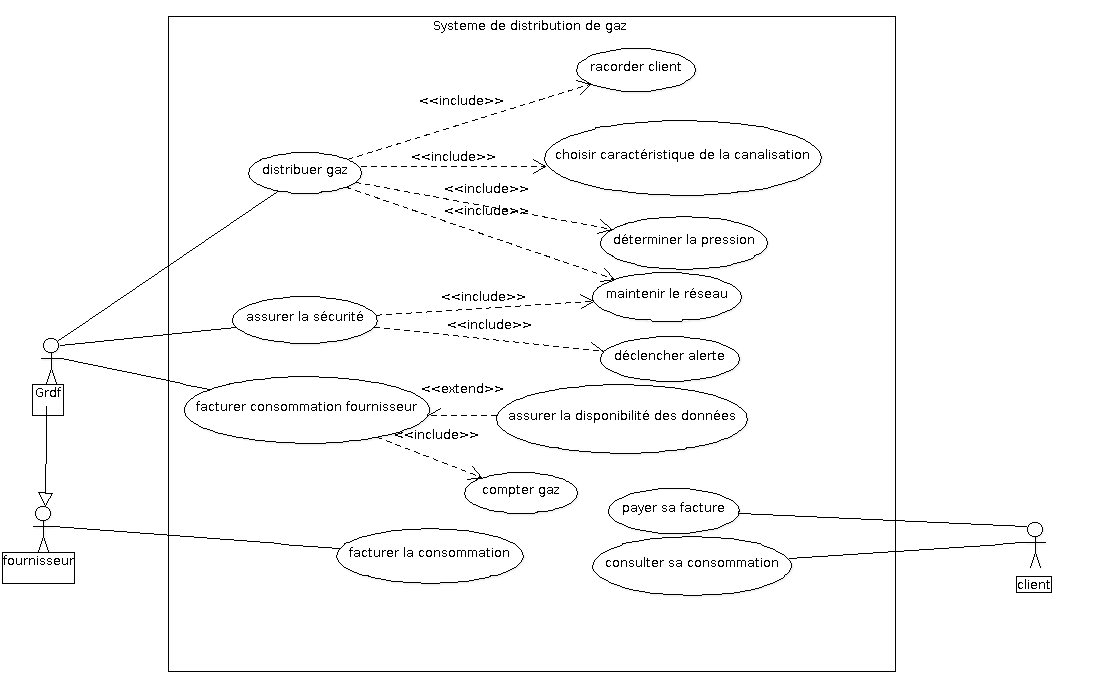
\includegraphics{Diagrammedecasdutilisation.png}
\caption{alt text}
\end{figure}

Les principales utilisations du réseau sont présentées à l'aide des
fiches suivantes :

\subsubsection{Titre : Interrompre la fourniture.}

\emph{Résumé} : Ce cas d'utilisation, permet à GrDF de couper le gaz
pour les clients qui n'ont pas payé leurs consommations suite à la
demande de leurs fournisseurs.

\emph{Acteurs} :

GrDF, fournisseur et client.

\emph{Préconditions} :

\begin{enumerate}[1.]
\item
  Client n'a payé sa facture.
\item
  le fournisseur demande à GrDF de couper le gaz pour le client
\item
  Un agent est disponible pour se déplaçer.
\end{enumerate}

\emph{Scénario nominal} :

\begin{enumerate}[1.]
\item
  si le contrat du client n'est pas soumis à une obligation de maintient
  de fourniture, le fournisseur demande un déplacement pour couper le
  gaz à GrDF.
\item
  GrDF renvoie les informations pour la mission d'interruption.
\item
  Si client paye sa facture entre temps , le fournisseur demande
  d'annuler la mission d'interruption à GrDF.
\item
  si la demande ne dépasse pas le délai, GrDF annule la mission.
\item
  le fournisseur informe le client pour qu'il ait la possibilité sa
  facture à l'opérateur GrDF.
\item
  GrDF envoie l'opérateur.
\item
  si le fournisseur choisit l'option d'interruption ferme.
\item
  si le client prouve le paiement de sa facture, l'opérateur GrDF
  informe le fournisseur.
\item
  si le client ne prouve pas le paiement.
\item
  si l'opérateur est confronté à un cas de force majeur, il informe le
  fournisseur.
\item
  sinon, l'opérateur ferme le robinet du compteur.
\item
  si le fournisseur choisit l'option d'interruption optionelle.
\item
  si le client est présent.
\item
  Si le client accepte de payer sa facture, l'opérateur informe le
  fournisseur.
\item
  sinon l'opérateur ferme le robinet de compteur.
\item
  si le client refuse de payer sa facuture, l'opérateur ferme le robinet
  du compteur.
\item
  si le client est absent, l'opérateur ferme le robinet du compteur.
\item
  GrDF facture le déplacement au fournisseur.
\end{enumerate}

\subsubsection{Titre : Assurer la sécurité.}

\emph{Résumé} :

Ce cas d'utilisation, permet à GrDF d 'assuer la sécurité du réseau .
\emph{Acteurs} :

GrDF.

\emph{Description des scénario} :

\emph{Préconditions} :

1.le réseau est mis en place.

2.déclenchement d'un alerte.

3.disponibilité des opérateurs dédiés à la maintenance et sécurité.

\emph{Scénario nominal} :

\begin{enumerate}[1.]
\item
  L'appelant repère un incident et décide d'appeler.
\item
  Si il appelle le Standard de GrDF, il y a un appel systématique au
  CTA-CDIS .
\item
  L'opérateur qui a répondu à l' appel fait évaluer la situation selon
  la grille PGR.
\item
  Sinon il appelle le standard CTA-CODIS, il y a aussi un appel
  systématique au standard de GrDF.
\item
  L'opérateur du standard du CTA-CODIS évalué la situation selon la
  grille PGR.
\item
  La situation est grave, déclenchement de la procédure renforcée( voir
  scénario procédure renforcée).
\item
  Si la situation est normale, GrDF envoie l'opérateur.
\item
  L'opérateur fait l'évaluation sur terrain.
\item
  Si l'évaluation est grave, déclenchement de la procédure renforcée.
\item
  Si la situation est normale, il fait les réparations.
\item
  CTA-CODIS envoie le COS .
\item
  Le COS évalue la situation sur le terrrain.
\item
  Si l'évaluation est grave, déclenchement de la procédure renforcée.
\item
  Sinon l'opérateur GrDF fait la réparation.
\end{enumerate}

\emph{Scénario nominal} (Procédure Renforcée).

1.COS prépare le plan d'intervention.

\begin{enumerate}[1.]
\setcounter{enumi}{1}
\item
  COS demande l'intervention des autres services (police, mairie,
  smur\ldots{}).
\item
  COS demande à l'opérateur GrDF d'identifier la canalisation.
\item
  l'opérateur GrDF interroge Carpathe pour identifier la canalisation.
\item
  Carpathe renvoie les données relatives à la canalisation.
\item
  Si la canalisation est de basse pression, l'opérateur GrDF effectue
  les réparations.
\item
  Si la canalisation est de moyenne pression, l'opérateur GrDF ferme les
  robinets.
\item
  l'opérateur GrDF dépressurise la canalisation.
\item
  l'opérateur GrDF répare la canalisation.
\end{enumerate}

Nous venons donc de décrire l'utilisation que nos acteurs, dans le champ
que l'on a délimité font du réseau de distribution. Sans pour autant
décrire chaque détails, nous allons expliquer comment le gaz est
acheminé depuis l'endroit où il se situe naturellement jusqu'au
consommateur.

\subsection{Transport du gaz}

Le gaz distribué par GrDF est un gaz dit naturel : il provient des
réserves souterraines ou sous-marines. Ces réserves de gaz sont le
résultat de la décomposition d'êtres vivants au cours du temps. Cette
décomposition passe par un phase de méthanisation. C'est à ce moment que
le gaz naturel se forme, sa composition chimique est CH4 (méthane). Le
gaz naturel est à opposer à ce que l'on appelait auparavant le gaz de
ville qui était produit par extraction du méthane contenu dans le
charbon. Cette activité est maintenant terminée.

\subsubsection{Titre : Transporter le Gaz.}

****mettre le diag\emph{*}

\emph{Résumé} : Ce cas d'utilisation à GrDF de distribuer le gaz aux
clients.

\emph{Acteur} : GrDF.

\emph{Description des scénario} :

\emph{Préconditions} :

\begin{enumerate}[1.]
\item
  il y a du gaz dans le réseau.
\item
  il y a des clients.
\end{enumerate}

\emph{scénario nominal} :

\begin{enumerate}[1.]
\item
  le gaz est dans le réseau.
\item
  si le gaz est liquide, il est gazéifié.
\item
  le gaz est comprimé
\item
  le mercaptan est injecté dans le gaz pour lui donner une odeur à la
  frontière.
\item
  le gaz est de nouveau comprimer afin qu'il puisse avancer dans les
  canalisations.
\item
  soit il est détendu en MPC.
\item
  soit il est détendu en MPB.
\item
  s'il a été détendu en MPC, il est de nouveau détendu en MPB.
\item
  soit il est détendu pour alimenter un poster client (souvent
  industriel ou commercial).
\item
  soit il est détendu afin d'alimenter un consommateur classique.
\item
  soit il est détendu en basse pression pour alimenter un client
  classique (réseau en fonte ductile, remplacement à venir).
\end{enumerate}

Suite au transport du gaz depuis les carrière naturel vient donc le
consommateur, auquel GrDF ne facture rien directement mais avec qui il a
tout de même certains liens.

\section{Relation avec le client}

\subsection{Raccordement de nouveaux clients}

Une des fonctionnalités du système de distribution de gaz est de pouvoir
ajouter de nouveaux clients et donc de nouveaux bâtiments au réseau de
gaz. Il faut pour cela réaliser éventuellement une extension de réseaux
puis un branchement, qui correspond à la liaison entre les canalisations
du réseau de gaz et le coffret individuel du particulier :

\begin{figure}[htbp]
\centering
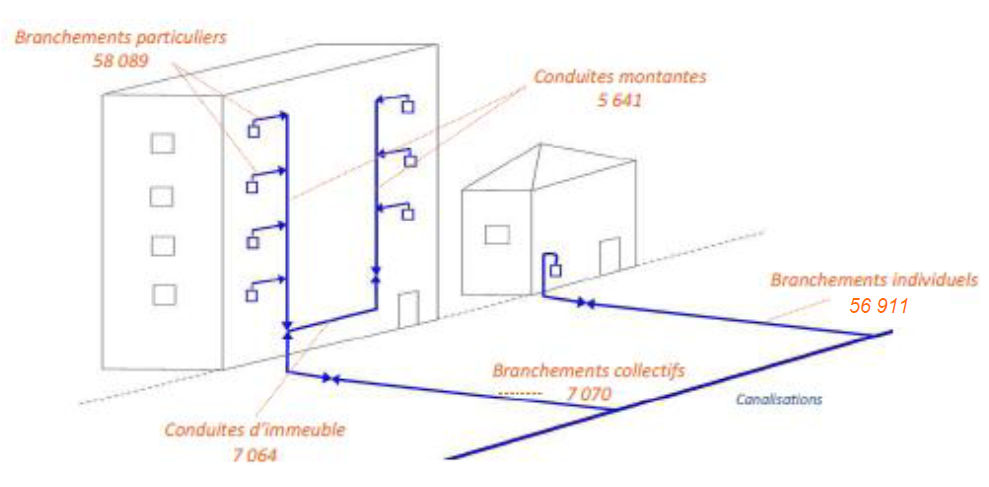
\includegraphics{branchementparticulier.png}
\caption{alt text}
\end{figure}

Représentation des branchements entre les canalisations et les
particuliers

En dépit des évolutions législatives et réglementaires, suite à la mise
en concurrence de l'énergie, Grdf reste responsable de la bonne
réalisation de la procédure de raccordement. Deux cas sont possibles :

\begin{itemize}
\item
  La maison est située à moins de 35 mètres du réseau de distribution de
  gaz naturel et l'usager peut bénéficier d'une offre de raccordement
  forfaitaire.
\item
  Dans le cas contraire, le raccordement fait l'objet d'un devis
  personnalisé.
\end{itemize}

Les travaux de raccordement nécessitent l'accord préalable des autorités
administratives compétentes (voir publique).

La procédure de branchement est la suivante :

\subsubsection{Scénario du branchement}

\emph{Cas d'utilisation} :

raccorder un nouveau client au réseau.

Ce cas d'utilisation permet de raccorder un nouveau client au réseau de
gaz.

\emph{Acteurs} :

Client, Distributeur, Fournisseur

\emph{Préconditions} :

Un nouveau client souhaite être raccordé au réseau de gaz.

\emph{Scénario nominal}

\begin{enumerate}[1.]
\item
  le client contacte directement le distributeur pour une demande de
  raccordement.
\item
  La maison est à moins de 35 mètres et le distributeur transmet donc au
  client un devis forfaitaire, de façon synchrone.
\item
  Le client donne son accord au distributeur et verse un acompte.
\item
  Le distributeur réalise à son niveau la planification des travaux de
  raccordement.
\item
  Le distributeur transmet le planning de réalisation des travaux de
  raccordement au client, afin qu'il donne son accord.
\item
  Le client donne son accord au distributeur concernant le planning de
  réalisation.
\item
  Le distributeur facture le solde au client.
\item
  Le client effectue le paiement du solde au distributeur.
\item
  Le distributeur transmet une demande de rendez-vous au client pour
  réaliser la mise en service.
\item
  Le client transmet son accord au distributeur.
\item
  Le distributeur réalise la mise en service.
\item
  Le distributeur réalise la mise à jour des différents S.I concerné par
  le raccordement (CARPATHE, OMEGA, DISCO).
\item
  Le distributeur procède au premier relevé d'index.
\item
  Le distributeur transmet alors l'index au fournisseur.
\item
  Le fournisseur envoie alors la première facture au client.
\end{enumerate}

\emph{Enchaînements alternatifs}

A1 : le client s'adresse directement au fournisseur. 1. Le client
souscrit un contrat de fourniture. 2. Le fournisseur mandate le
distributeur pour une demande de raccordement. A2 : la maison est située
à plus de 35 mètres du réseau de gaz. 4. Le distributeur fixe un
rendez-vous au client pour réaliser l'étude appropriée. 5. Le client
donne son accord à la demande de rendez-vous. 6. Le distributeur réalise
le devis personnalisé. 7. Le distributeur transmet le devis au client.

\emph{Post conditions} :

Le client peut désormais utiliser le gaz naturel, tant qu'il paye ses
factures.

\begin{figure}[htbp]
\centering
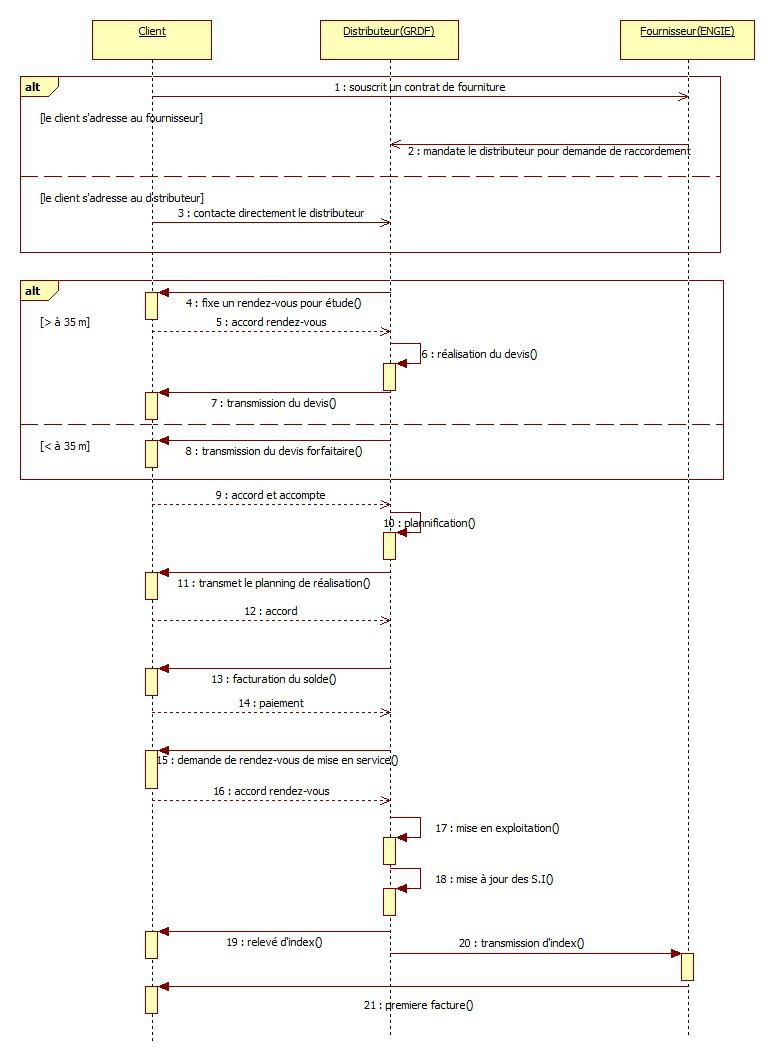
\includegraphics{sequenceraccordement.jpg}
\caption{alt text}
\end{figure}

Comme les travaux de raccordement s'arrêtent au niveau du coffret de
comptage du particulier, un installateur viendra par la suite sur place
pour relier la maison et mettre en place les équipements intérieurs
(pose de la canalisation reliant le coffret de comptage à la maison,
mise en route des appareils de chauffage\ldots{}).

Bien sûr GrDF intervient pour relier le consommateur au réseau, mais
GrDF intervient aussi pour couper l'accès du client au gaz.

\subsection{Interruption}

\begin{figure}[htbp]
\centering
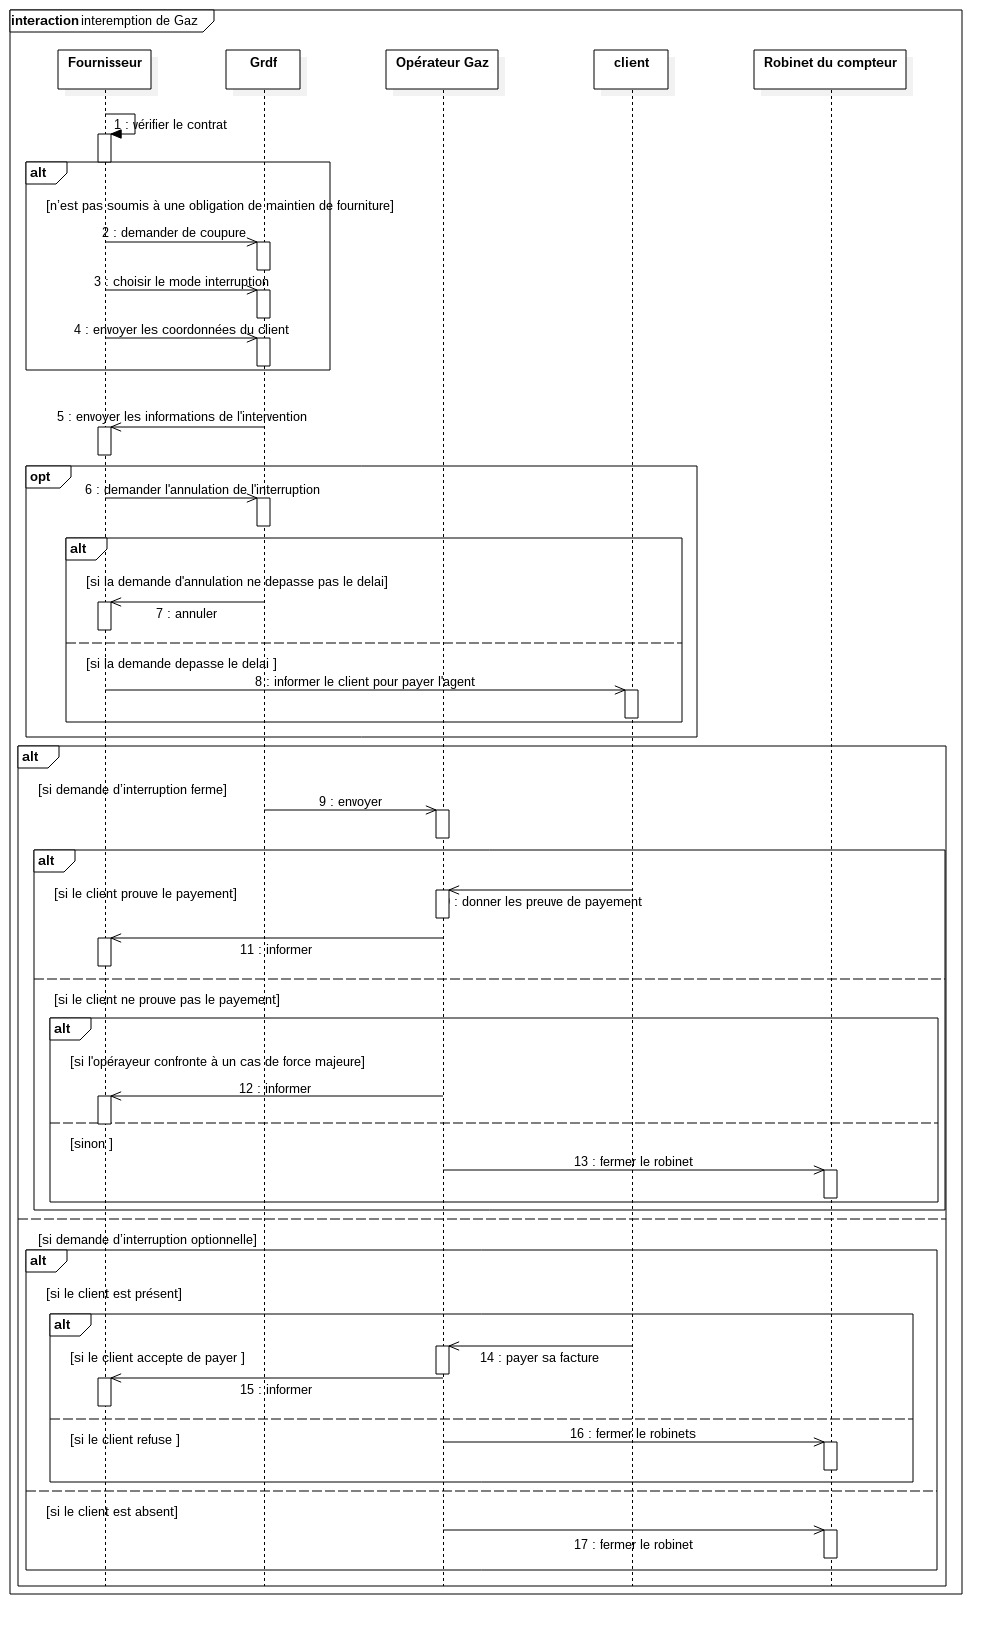
\includegraphics{DS-interruptionFournitureGaz.jpg}
\caption{alt text}
\end{figure}

Le graphique précédent présente la séquence amenant l'interruption de
fourniture du gaz à un consommateur.

Tout d'abord il faut voir si il y a une obligation de maintien de
fourniture. Cette obligation est décrite dans le décret n° 2008-780 du
13 août 2008 relatif à la procédure applicable en cas d'impayés des
factures d'électricité, de gaz, de chaleur et d'eau.

Dans le cas où il n'y a pas obligation de maintien de fourniture, le
fournisseur envoie les informations à propos de la mission
d'interruption de fourniture du gaz. Suite à cela GrDF envoie les
informations concernant l'intervention.

Il est possible que le fournisseur demande l'annulation de
l'intervention. Dans ce cas, soit cette demande d'annulation ne dépasse
pas le délai d'attente et l'intervention est annulée, soit le
fournisseur informe son client de l'intervention d'interruption de
fourniture et lui laisse la possibilité de payer l'agent.

L'opérateur GrDF est donc envoyé chez le client. Une nouvelle fois deux
cas sont possibles :

\begin{itemize}
\item
  Soit la demande d'interruption est ferme.
\item
  Soit c'est une demande d'interruption optionnelle.
\end{itemize}

Dans le cas d'une demande d'interruption ferme, soit le client prouve
qu'il a bien payé sa facture à l'opérateur GrDF qui en informe alors le
fournisseur, soit il ne peut pas prouver qu'il a payé,. Si l'opérateur
est confronté à un cas de force majeur et en informe alors le
fournisseur, soit il ferme simplement le compteur du robinet de gaz.

Dans le cas d'une demande d'interruption optionnelle, soit le client est
présent et a alors la possibilité de payer sa facture à l'opérateur qui
peut prendre cette opportunité ce qui conduit l'opérateur à en informer
le fournisseur. Il est aussi possible qu'il ne soit pas en mesure de
payer, son robinet du compteur de gaz est alors fermé par l'opérateur.

En cas d'absence du client, son robinet est fermé par l'opérateur. Suite
à cela, GrDF facture à l'intervention au fournisseur.

\section{Transmission des données et sécurité}

\subsection{Gazpar, le compteur communiquant}

\subsubsection{L'état actuel du système de comptage}

Actuellement, l'écrasante majorité des compteurs de gaz ne sont pas «
intelligents » et nécessitent l'intervention d'un opérateur tous les 6
mois pour relever la consommation effective.

l'intervention d'un opérateur tous les 6 mois pour relever la
consommation effective.\\Depuis 50 ans, le système de comptage n'a donc
pas tellement évolué. Il est en effet basé sur un dispositif à membranes
: la membrane, mobile et étanche au gaz, de chaque compartiment est mise
en mouvement par la différence de pression entre l'amont et l'aval du
compteur. Les tiroirs de distribution admettent le gaz alternativement
d'un côté de la membrane, puis de l'autre et d'un compartiment à
l'autre. Les deux membranes sont reliées chacune à un embiellage qui
transforme le mouvement alternatif des soufflets en un mouvement de
rotation continu entraînant le totaliseur mécanique, selon la figure
suivante :

\textbf{\emph{figure à définir}}

Image dispositif de comptage.

Ce dispositif est resté en l'état sur les compteurs les plus récents,
qui possèdent seulement en plus une sortie exploitable pour les
traitements électroniques. Toutefois, même si ce système de comptage
reste fiable, il n'en demeure pas moins contraignant pour le
distributeur qui est obligé de se déplacer pour relever la consommation
tous les six mois, ainsi que pour le client qui doit être présent à ce
moment. C'est pourquoi, d'autres systèmes de comptage sont actuellement
à l'étude.

\subsubsection{Le système Gazpar}

La phase de lancement du projet de compteur communicant, appelé GAZPAR,
a vu le jour à la fin de l'année 2009, suite à la délibération de la
Commission de Régulation de l'Energie (CRE) du 3 septembre 2009. Ce
projet s'inscrit dans la politique de modernisation de GrDF débutée en
2004. Il est favorisé par le contexte institutionnel et réglementaire,
en effet, une directive du conseil de l'Union Européenne de 2008 demande
la mise à disposition des informations sur les consommations de gaz aux
consommateurs. Il a pour objet de faire remonter des informations en
direct concernant notamment l'index de consommation du foyer dans lequel
il est installé, pour une facturation sur la consommation réelle.

\begin{figure}[htbp]
\centering
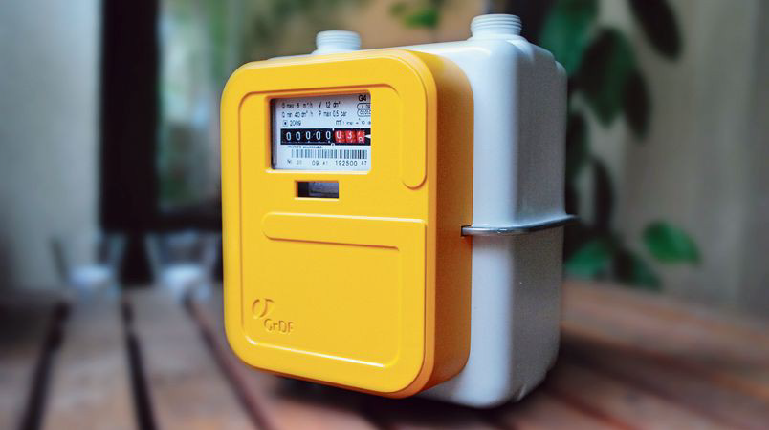
\includegraphics{compteurgazpar.png}
\caption{alt text}
\end{figure}

Ce projet fait suite aux attentes des clients d'être facturés sur des
index réel et non plus sur des estimations de consommations. D'autre
part, l'accès à une donnée de consommation réelle et fréquente est un
prérequis pour les autorités pour mieux sensibiliser à la maîtrise de la
demande en énergie. Enfin, la modernisation des infrastructures
améliorera la réactivité du fournisseur et du distributeur. En effet,
une meilleure connaissance des quantités de gaz acheminées et consommées
permettra l'optimisation de la gestion des réseaux de gaz.

Selon, les résultats de la consultation publique menée par la CRE en
2011, les fonctionnalités principales retenues sont les suivantes :

\begin{itemize}
\item
  Paramétrage du compteur en local
\item
  Supervision de l'infrastructure de télé relève
\item
  Prise en compte de demandes d'index faites par les fournisseurs
\item
  Consommation réelle à périodicité mensuelle
\item
  Modification ponctuelle du pas de mesure (pas horaire)
\end{itemize}

Le projet prévoit donc entre autre d'équiper ou de remplacer près de 11
millions de compteurs d'ici à 2022. GrDF estime que 10\% des compteurs
assez récents pourront être équipés d'un module radio pour la
transmission des index de consommation et que les 90\% restant seront
remplacés par de nouveaux compteurs composés entre autre d'un module
radio. Concrètement, la mise en œuvre du système de comptage évolué
consiste à :

\begin{itemize}
\item
  Concevoir et construire une solution technique de télé relevé basée
  sur une solution de réseau radio fixe et des Systèmes d'Information
  (SI) permettant de collecter les données de consommation et
  d'effectuer le calcul d'énergie ;
\item
  Déployer sur l'ensemble du territoire, environ 15 000 concentrateurs,
  d'après les études radio réalisées, maillons essentiels de la chaîne
  communicante, positionnés sur les points hauts. *- Equiper ou
  remplacer près de 11 millions de compteurs d'ici à 2022. Environ 10\%
  des compteurs les plus récents seront équipés de modules radio
  déportés (voir figure suivante), les 90\% restants seront quant à eux
  remplacés par des « compteurs communicant gaz » équipés de modules
  radio intégrés.
\end{itemize}

\begin{figure}[htbp]
\centering
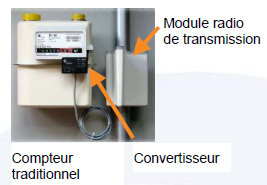
\includegraphics{module.png}
\caption{alt text}
\end{figure}

Image module de transmission radio à brancher

Comme illustré sur la figure précédente, les compteurs les plus récents
seront simplement équipés de module de transmission radio, qui sera
composé principalement d'un quartz et d'une antenne et d'une pile,
sensée durer 20 ans :

\begin{figure}[htbp]
\centering
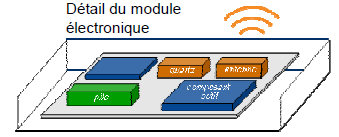
\includegraphics{detailmodule.png}
\caption{alt text}
\end{figure}

(Image de détail du module électronique à brancher)

Le fonctionnement de la chaîne communicante est décrit sur le schéma
suivant :

\begin{figure}[htbp]
\centering
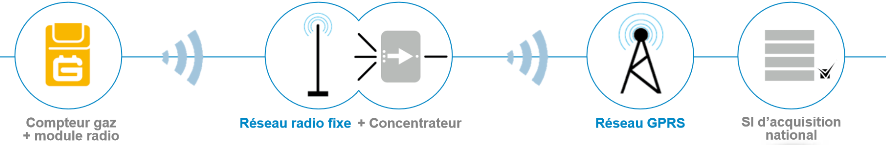
\includegraphics{chainemodule.png}
\caption{alt text}
\end{figure}

Deux fois par jour, et à raison de quelques secondes à chaque fois, le
compteur Gazpar rentre en communication par ondes radio avec un
concentrateur situé dans le voisinage sur un point haut afin de
l'informer du dernier relevé de consommation. Chaque concentrateur
collecte les informations de tous les compteurs Gazpar environnants et
les retransmet à son tour, via le réseau GPRS (les concentrateurs
possèdent de leur côté une carte SIM), à un centre national de
supervision.

Pour d'évidentes raisons de sécurité relatives au caractère personnel
des index de consommation et en accord avec la CNIL, les échanges de
données sont sécurisés via un algorithme de chiffrement symétrique : AES
128. Le choix d'un algorithme symétrique se justifie par le fait que les
communications doivent être rapides.

Lors de la communication du compteur vers le concentrateur, les données
sont donc chiffrées puis transmises par ondes radio, à la fréquence de
169 MHz, en réseau local (LAN) aux deux concentrateurs les plus proches.
La fréquence de 169 MHz correspond en France à la transmission de
mesure, elle a été choisie par rapport la fréquence d'usage libre de 868
MHz, car à puissance égale une transmission à 169 MHz portera 5 fois
plus loin qu'une émission à 868 MHz. Donc dans un souci de préserver la
durée de vie de la pile et d'éviter d'avoir à installer d'éventuels
répéteurs, ce qui rendrait le projet trop onéreux, la fréquence de 169
MHz apparaît optimale.

Une fois arrivées au concentrateur, les données sont ensuite
retransmises au S.I d'acquisition national AMR (Automated Meter
Reading). Lors de cette communication, les données (index et état des
batteries) sont cette fois transmises via le réseau GRPS, en réseau
étendu (WAN). La transmission GPRS a été cette fois choisie à cause de
sa bande passante supérieure à celle du GSM. Le protocole de
transmission du réseau GPRS est par ailleurs basé sur le protocole de
communication TCP/IP (les concentrateurs possèdent en effet des adresses
IP privatives).

\begin{figure}[htbp]
\centering
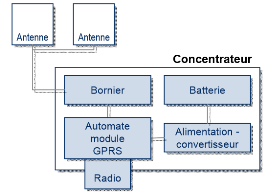
\includegraphics{compositionconcentrateur.png}
\caption{alt text}
\end{figure}

Schéma composition d'un concentrateur

En outre, la transmission des index de consommation a lieu 2 fois par
jour et ne se déroule pas forcément tous les jours à heure fixe.

En outre, la transmission des index de consommation a lieu 2 fois par
jour et ne se déroule pas forcément tous les jours à heure fixe. Pour
équiper ou remplacer les 11 millions de compteurs existants, GrDF a
prévu un planning de cinq ans, de 2017 à 2022. Il est pour cela prévu
d'installer de nouveaux systèmes d'information pour faciliter le
déploiement (voir le paragraphe suivant), ainsi que de dédier des
équipes à la pose de nouveau compteur. La pose du nouveau compteur fera
l'objet d'un rendez-vous, fixé en accord avec le client un mois en
amont. L'opérateur aura à sa disposition un outil de mobilité le
renseignant sur les différentes opérations à réaliser sur le compteur,
selon la figure suivante :

\begin{figure}[htbp]
\centering
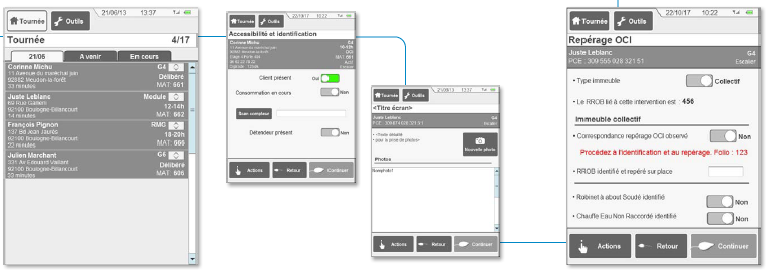
\includegraphics{outil.png}
\caption{alt text}
\end{figure}

Comme illustré ci-dessus, l'outil donnera des informations au technicien
sur le type d'intervention à réaliser pour chaque client (ex : organe de
coupure individuel ou pas ?). Le technicien de pose s'appuiera sur
celui-ci pour être guidé sur les gestes techniques à adopter lors de son
intervention ; cet outil devrait lui permettre de réaliser environ 16
interventions chaque jour.

\subsubsection{Traitements des index de consommation}

Pour chacun des 11 millions de compteur communicants qui seront
prochainement installés sur l'ensemble du territoire, GrDF va récupérer
2 relevés de consommation quotidiens. Ce qui représente un flux de
données conséquent et nécessite donc la mise en place de nouveaux
systèmes d'information ainsi que la mise à jour des systèmes
d'information existants. Les différents systèmes d'information concernés
ainsi que leurs interactions entre eux sont représentés sur la figure
suivante :

\begin{figure}[htbp]
\centering
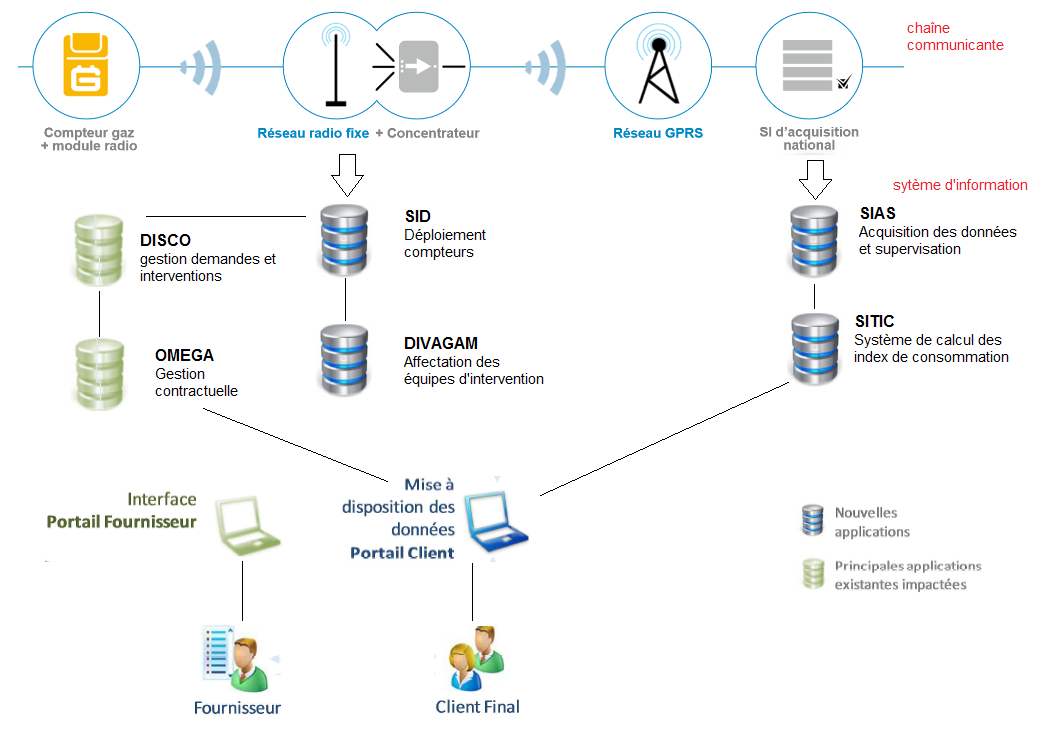
\includegraphics{sigazpar.png}
\caption{alt text}
\end{figure}

Déploiement de la solution de comptage

D'après le schéma précédent, les S.I mis en place avant l'apparition de
Gazpar, OMEGA et DISCO ont dû être mis à jour. En effet, le rôle d'OMEGA
est de mettre à disposition auprès des fournisseurs de gaz et des
gestionnaires de réseau de transport, en temps réel, les informations
relatives aux interventions et les mesures associées. Le système donc dû
s'adapter à une volumétrie importante puisqu'il gèrera désormais environ
11 millions de personnes et qu'il traitera 10 000 à 15 000 demandes par
jour.

\emph{Cas d'utilisation} :

collecter les données de consommation du client.

Ce cas d'utilisation permet de collecter les données de consommation du
client.

\emph{Acteurs} :

Technicien (principal), compteur (secondaire), concentrateur
(secondaire), AMR (secondaire), DISCO (secondaire), SITIC (secondaire),
SID (secondaire), DIVAGAM (secondaire)

\emph{Préconditions} :

on se situe à l'heure de relève automatique quotidienne de la
consommation de gaz.

\emph{Scénario nominal}

\begin{enumerate}[1.]
\item
  Le compteur chiffre les index de consommations.
\item
  Le compteur transmet les index chiffrés à deux concentrateurs
  habituels via des ondes radio à 169 MHz en réseau local (LAN).
\item
  Le concentrateur vérifie la véracité des informations.
\item
  Le concentrateur retransmet les informations au S.I d'acquisition
  national via le réseau GPRS en réseau étendu (WAN).
\item
  Le système d'acquisition déchiffre les informations.
\item
  Le système d'acquisition transmet les informations au système de
  calcul des index de consommation (SITIC).
\item
  SITIC calcule les index de consommation.
\item
  SITIC transmet les données à DISCO.
\item
  Mise à disposition des données à OMEGA en vue d'une facturation
  ultérieure.
\item
  Mise à disposition des données de consommation du client.
\item
  Mise à disposition des données de consommation au fournisseur.
\end{enumerate}

\textbf{\emph{Diagramme gazpar}}

Comme les travaux de raccordement s'arrêtent au niveau du coffret de
comptage du particulier, un installateur viendra par la suite sur place
pour relier la maison et mettre en place les équipements intérieurs
(pose de la canalisation reliant le coffret de comptage à la maison,
mise en route des appareils de chauffage\ldots{}).

Comme illustré sur le diagramme de séquence représentant la collecte des
données de consommation, ces informations doivent être mises à
disposition du client quotidiennement et doivent également être mise à
disposition du fournisseur.

Cette chaîne d'événements ne pourraient avoir lieux sans un réseau sûr,
c'est pourquoi nous allons préciser comment le réseau est mis en
sécurité.

\subsection{Sécurité du réseau}

Sur le réseau de GrDF, il y a certaines pièces mécaniques (robinet de
gaz, pièce contenu dans les postes de détente\ldots{}). Du fait de leur
fonctionnement mécanique, ces pièce sont plus soumises à l'usure que les
autres, cela implique une maintenance et une vigilance plus grande sur
celles-ci. En plus des pièces soumises à un usure mécanique naturelle,
il est possible qu'il y ait des fuite ailleurs sur le réseau. Afin de
détecter des éventuelles fuites sur le réseau, GrDF à mis en place des
véhicules munis de capteurs permettant de connaître la composition de
l'air et notamment la teneur en méthane, possible indicateur de fuite de
gaz. Les données récoltées par ces véhicules, croisées avec
l'incidentologie et le données contenues dans le SIG de GrDF permettent
de mettre en évidence les zones à moderniser sur le réseau.

Enfin, il est aussi possible que ce soit une tierce personne qui
découvre une fuite. Dans ce dernier cas un standard est ouvert à GrDF
afin de signaler l'incident. Le diagramme suivant décrit la séquence
d'action lors d'un appel.

\begin{figure}[htbp]
\centering
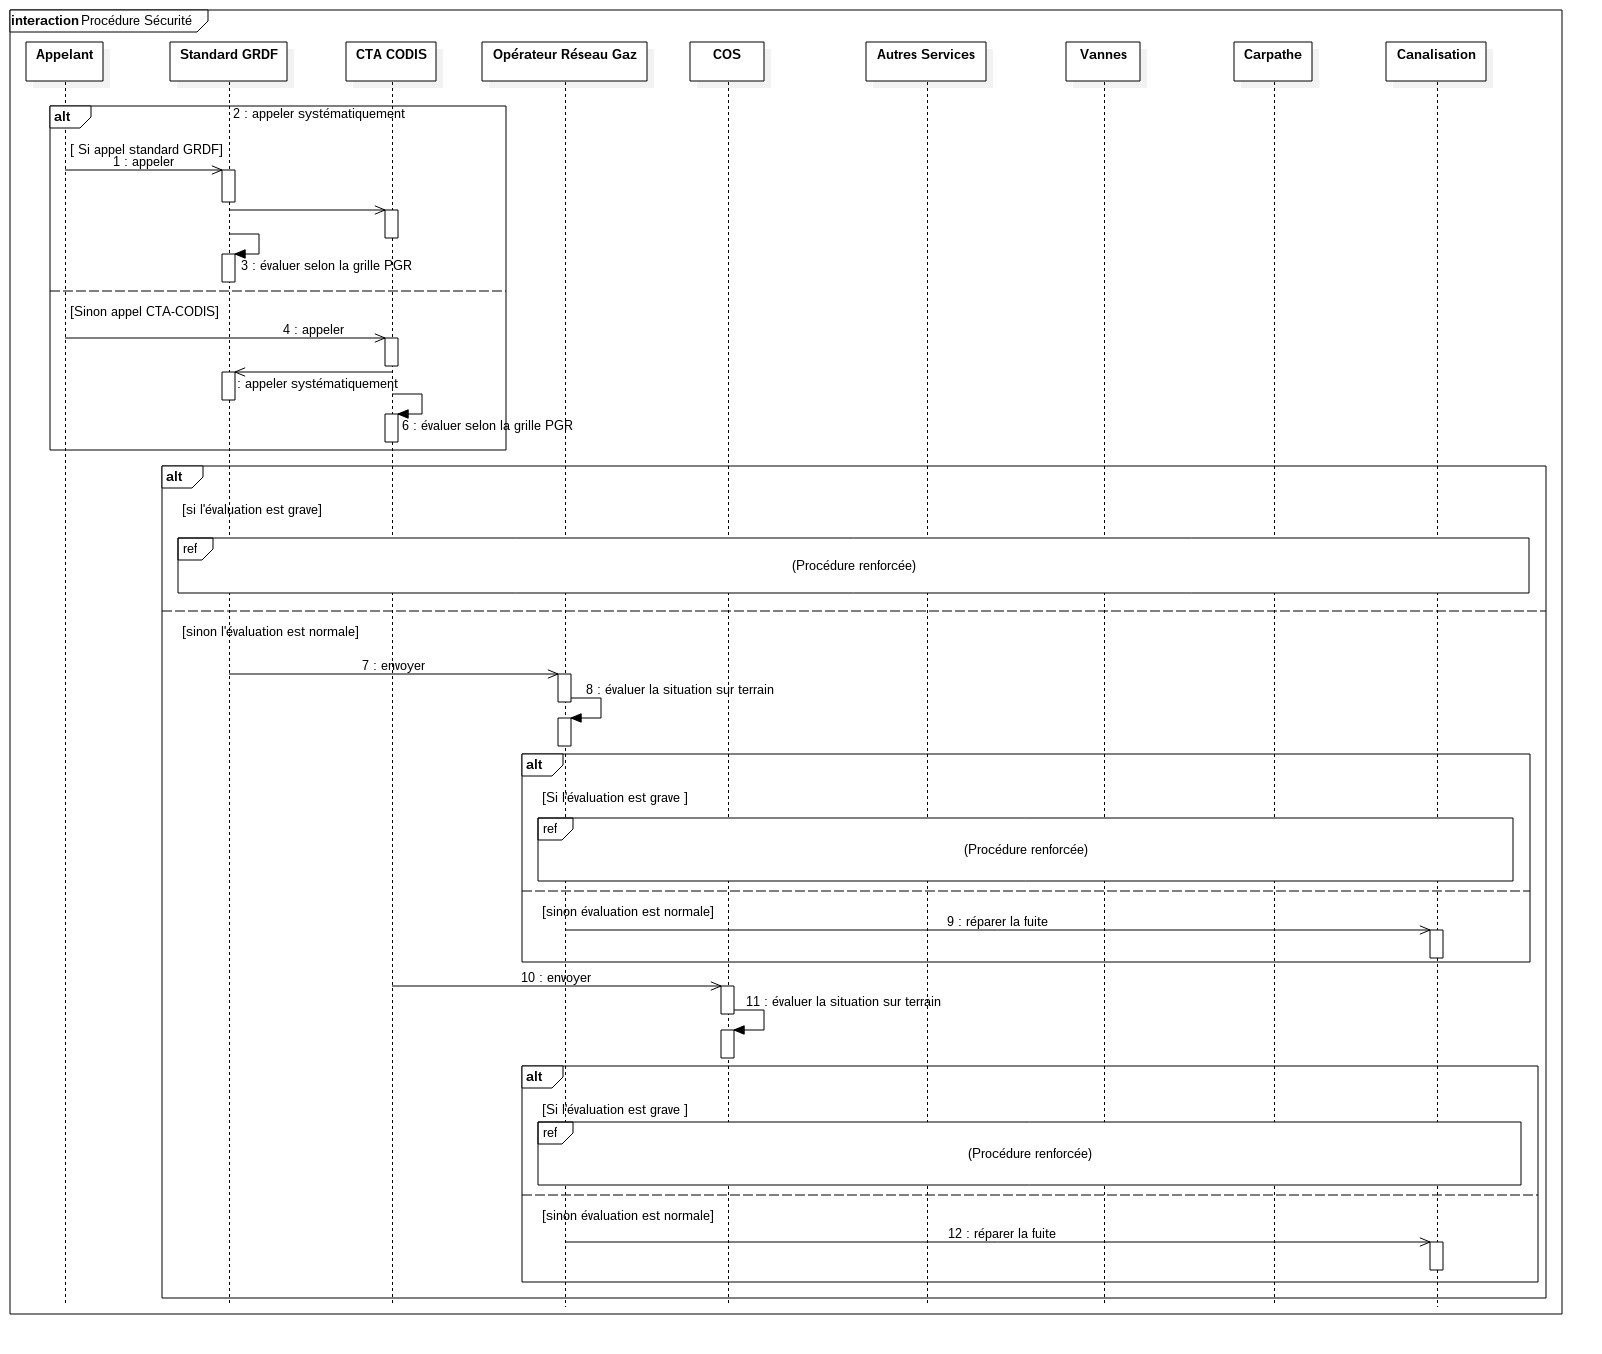
\includegraphics{DS-Securite.jpg}
\caption{alt text}
\end{figure}

Il est possible pour un appelant d'appeler le standard de GrDF ou le
centre de traitement des alertes des pompiers. Si c'est le standard de
GrDF qui est appelé, celui-ci relaie systématiquement l'appel aux
pompiers et la situation est évaluée par téléphone.

Dans le cas où ce sont les pompiers qui sont appelés, l'appel est relayé
à GrDF et la situation est évaluée selon les mêmes critères.

Si la situation est jugée comme étant grave, il y a lancement de la
procédure renforcée. Cette dernière est décrite dans le diagramme
suivant.

\begin{figure}[htbp]
\centering
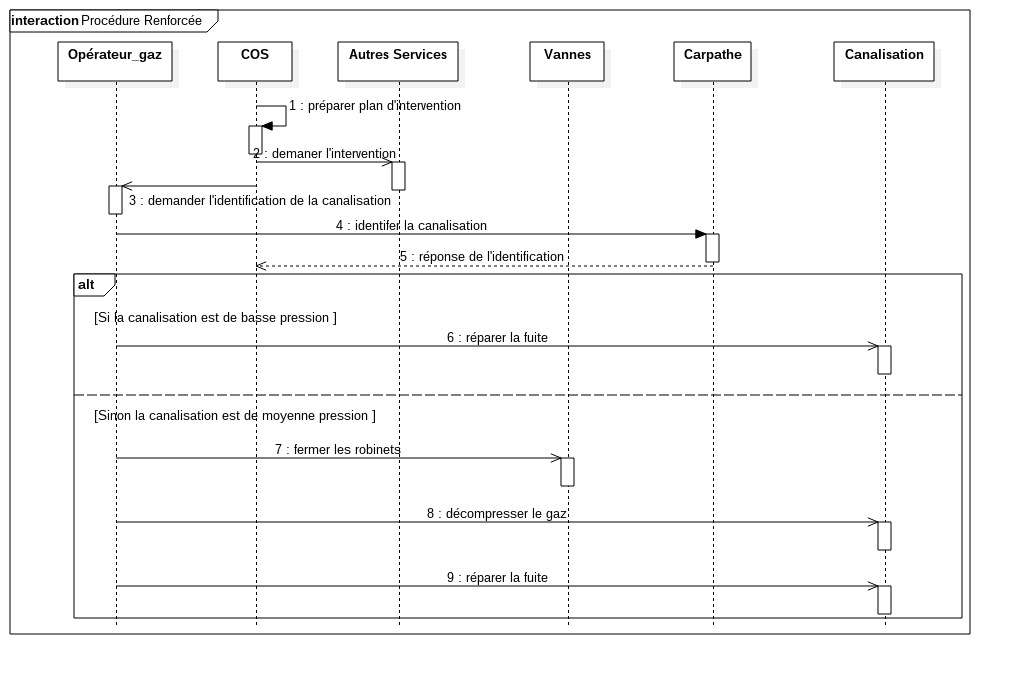
\includegraphics{Ds_ProcedureRenforcee.jpg}
\caption{alt text}
\end{figure}

Lorsque la procédure renforcée est lancée, les pompiers prépare le plan
d'intervention puis demande l'intervention d'autres services (smur,
police\ldots{}). Ils demandent ensuite l'identification de la
canalisation par un opérateur GrDF. Cet opérateur interroge ensuite
l'outil Carpathe afin d'identifier la canalisation puis donne la réponse
aux pompiers.

Si la canalisation est en basse pression alors l'opérateur répare la
canalisation. Si elle est en moyenne pression, l'opérateur ferme les
robinets de gaz alimentant la zone où a lieu la fuite, décompresse la
canalisation puis la répare.

Dans le cas où l'évaluation est normale, la situation est de nouveau
évaluée sur le terrain par l'opérateur GrDF. Si la situation est jugée
grave, la procédure renforcée est lancée, dans le cas contraire la
canalisation est réparée. De même les pompiers sont envoyés sur le
terrain, et procèdent à une évaluation. Une nouvelle fois, si la
situation est grave, la procédure renforcée est lancée, sinon la
canalisation est réparée.

\section{Synthèse}

\begin{figure}[htbp]
\centering
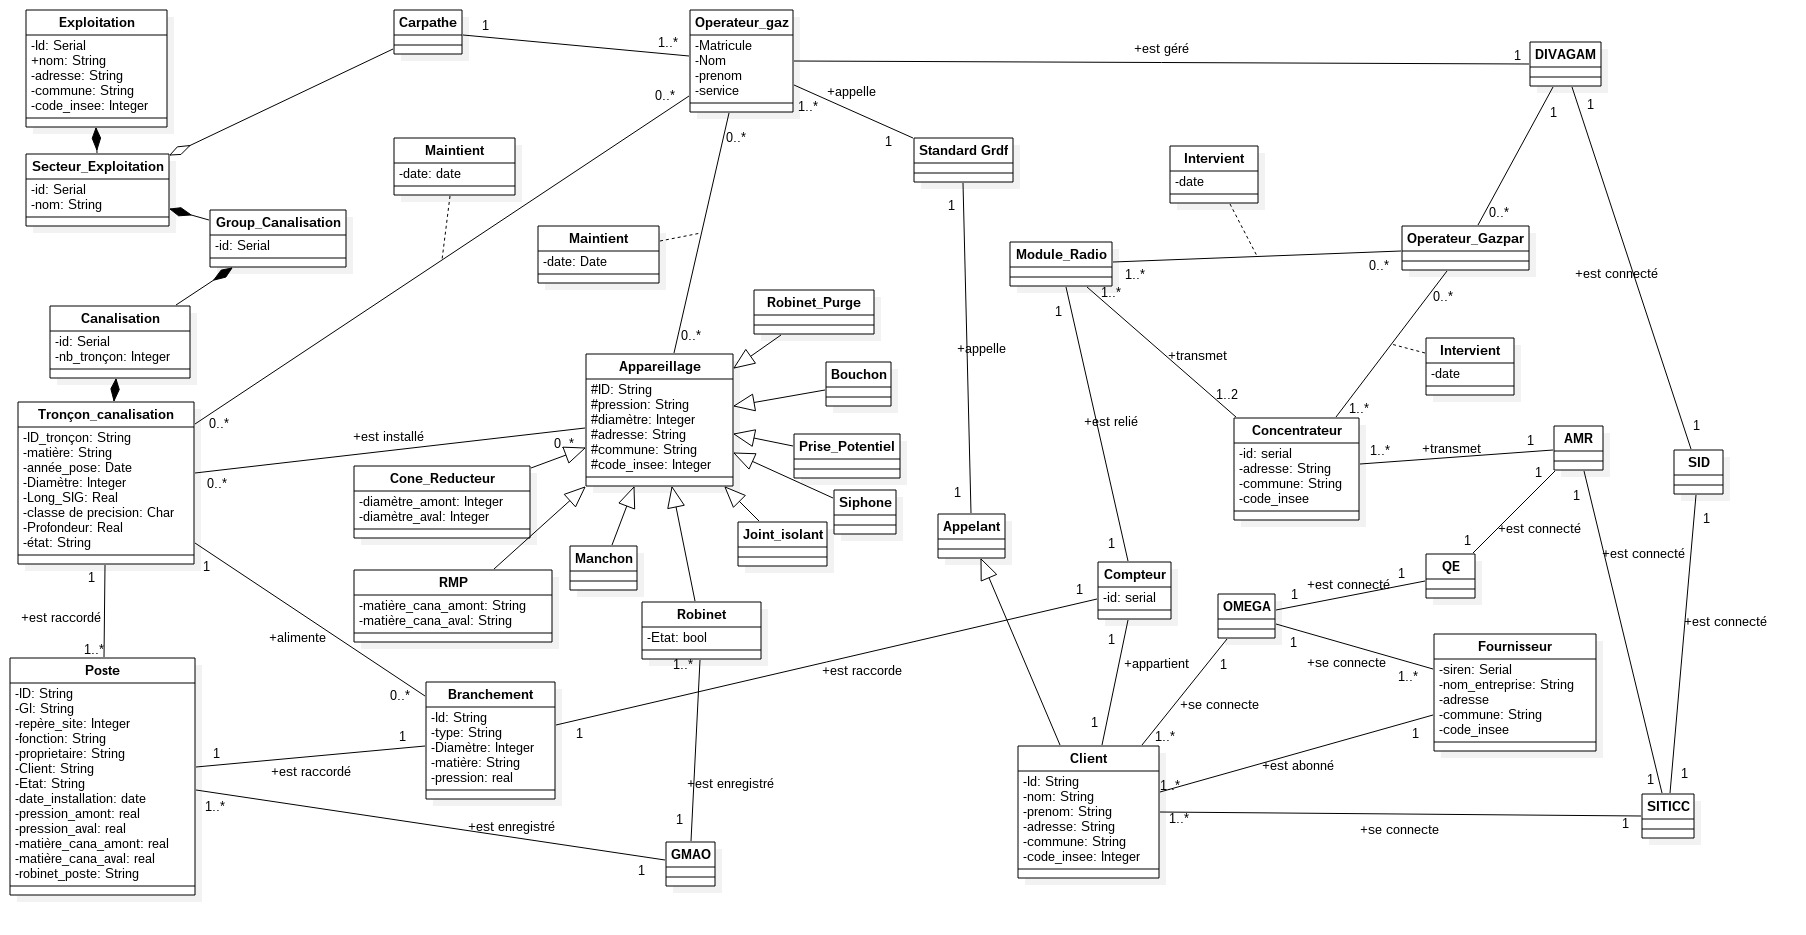
\includegraphics{D-Classe.jpg}
\caption{alt text}
\end{figure}

Le diagramme du classe ci-dessus met en lien les différentes partie du
rapport précédemment présentées. Y figure les principaux attributs de
chaque classe.

Dans cette dernière partie on se focalisera sur la partie SIG de GrDF,
le reste ayant été traité précédemment dans le rapport.

Du point de vue du SIG de GrDF, la classe la plus utilisée est le
tronçon de canalisation. Celui-ci possède des attributs qui permette de
le définir : sa matière, son année de pose\ldots{} Ces Tronçons de
canalisation peuvent être reliés à des postes. Ces postes peuvent être
des postes clients (grand consommateur de gaz) ou des postes de détente.
Si on a un client classque et pas un postre client, le tronçon de
canalisation est en lien avec un branchement qui relie le tronçon au
compteur. Le compteur est ensuite relié au système d'envoie de données
comme présenté dans les parties précédentes. Ces Tronçons de
canalisation sont aussi à relier à l'appareillage, en effet, c'est bien
sur ces tronçons que seront reliés les différents manchons, robinets,
etc\ldots{}

Au dessus des tronçons de canalisation, on trouve la canalisation qui
est une composition de tronçons.

De même une composition de canalisations forment un groupe de
canalisation.

Une aggrégation de groupes de canalisations forment un secteur
d'exploitation.

Enfin, plusieurs secteurs d'exploitation se trouvant sur une même zone
géographique forment une exploitation.

\section{Bibliographie et sitographie}

\begin{itemize}
\item
  Note d'information opérationnelle, Intervention pour fuite sur
  unréseau de gaz naturel, Ministère de l'Intérieur Procédure pour
  déplacement impayé, GrDF
\item
  Projet compteurs communiquants gaz de GrDF, GrDF
\item
  Projet compteurs communicants gaz, prestations de pose des nouveaux
  compteurs communiquants Gazpar, GrDF
\item
  Prescriptions techniques applicables aux canalisations de transports
  de GRTgaz et aux installations de transport, de distribution et de
  stockage de gaz raccordés au réseau de GRTgaz.
\item
  Etude comptage évolué gaz, Sopra Consulting
\end{itemize}

% 6 - backmatter
\end{document}
